% !TeX root = ../main.tex

\section{Exercises}

\subsection{20220217-1}
    A signal $x[n]$ is filtered using a filter $h[n]$ that is the cascade of two filters, $h_1[n]=\brackets{1,-1}$ and $h_2[n]=\brackets{1,0,4}$

    \subsubsection{Temporal sequence, convolution and z-transform}
    1. [3 pts] Find the temporal sequence of the filter $h[n]=\cdots$ and its z-transform $H(z)=\cdots$

    \mybox{
        $$
        y(n)=x(n)*h(n)=\sum_{k=-\infty}^\infty x(k)h(n-k)
        $$
        The convolution:
        \begin{itemize}
            \item Flip the second term $h(n)\rightarrow h(-k)$
            \item Shift $h$ by adding $n$ (if positive shift to right, if negative to left) $h(n-k)$
            \item For output $y(n)$ sum all contributions of $x(k)$ and the shifted flipped $h$
        \end{itemize}
        Last step similar to scalar product. \textbf{The length of the convolution is the sum of the two signals-1 and the support (x-axis from when the signals start to differ from 0) is the sum of the supports until the final support of the two}

        So in our case the length of the convolution is $2+3-1=4$. We first flip $h_2$ then
        \vspace{1em}
        
        $
        h[n=0]=
        \begin{Bmatrix}
                &       & 1     & -1\\
            \cdot & \cdot & \cdot & \cdot \\
            4     & 0     & 1
        \end{Bmatrix}=1\\
        \\
        h[n=1]=
        \begin{Bmatrix}
                & 1     & -1\\
            \cdot & \cdot & \cdot \\
            4    & 0     & 1
        \end{Bmatrix}=-1\\
        \\
        h[n=2]=
        \begin{Bmatrix}
            1     & -1\\
            \cdot & \cdot & \cdot\\
            4     & 0     & 1
        \end{Bmatrix}=4\\
        \\
        h[n=3]=
        \begin{Bmatrix}
            1     & -1\\
            \cdot & \cdot & \cdot & \cdot\\
                & 4     & 0     & 1
        \end{Bmatrix}=-4
        $

        \vspace{1em}
        So $h[n]=\brackets{1,-1,4,-4}$. Its z-transform:
        $$
        H(z)=1-z^{-1}+4z^{-2}-4z^{-3}
        $$
        Alternatively, we apply the distributive property of the convolution. Consider:
        $$h_2[n]=\delta[n]+4\delta[n-2]$$
        So
        $$
        h[n]=h_1[n]*\delta[n]+h_1[n]*4\delta[n-2]=h_1[n]+4h_1[n-2]=
        $$
        $$
        \Brackets{1,-1,0,0}+4\Brackets{0,0,1,-1}=\Brackets{1,-1,4,-4}
        $$
    }

    \subsubsection{Pole-zero plot and magnitude}
    2. [3 pts] Represent the pole-zero plot of $H(z)$ and its magnitude.

    \mybox{
        We must rewrite $H(z)$ into a fraction:
        \vspace{1em}

        $
        H(z)=1-z^{-1}+4z^{-2}-4z^{-3}=1-\frac{1}{z}+4\frac{1}{z^2}-4\frac{1}{z^3}=
        \\=\cdots\frac{1}{z^3}\left(z^3-z^2+4z-4\right)
        $

        \begin{center}
            \begin{tabular}{c| c c c|c}
                & 1 & -1 & 4 & -4 \\
                1 &   &  1 & 0 &  4 \\ \hline
                & 1 &  0 & 4 &  0
            \end{tabular}        
        \end{center}

        $
        \\=\cdots\frac{\left(z-1\right)\left(z^2+4\right)}{z^3}
        $
        
        \vspace{1em}
        So we have:
        \begin{itemize}
            \item \textbf{Three poles} in $0$
            \item \textbf{A zero} in $1$
            \item \textbf{Two complex conjugate zeros} in $\pm 2j$
        \end{itemize}
        We notice that the filter is FIR, it has only poles at the origin.
        \begin{center}
            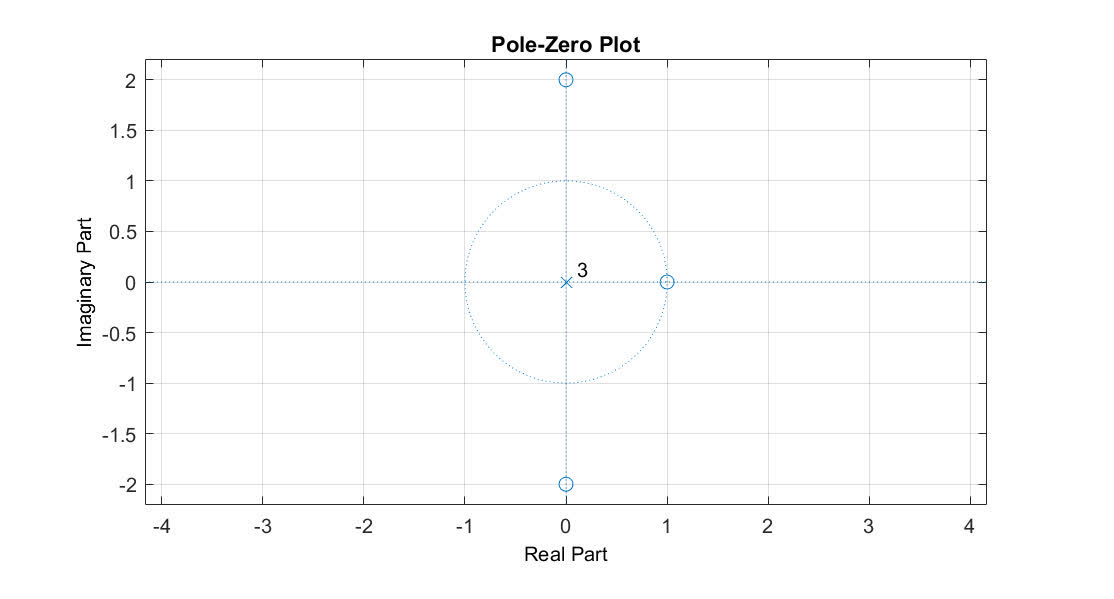
\includegraphics[width=1\textwidth]{images/20220217_01.png}
        \end{center}
        For the amplitude we just look at the pole-zero plot and multiply all origin-zero distances while we divide for all origin-pole distances. As all the poles are at the origin, their distance from a point on the circle will always be 1. We plot from 0 to $\pi$ as $-\pi$ to $0$ is symmetric, so normalized in $0$ to $1$. As $z=\rho e^{j2\pi f}=e^{j\omega}$:
        \begin{itemize}
            \item $\omega=0,\,\,z=1\rightarrow|H(z)|=0$
            \item $\omega=\frac{\pi}{2},\,\,z=j\rightarrow|H(z)|=3\sqrt{2}\sim 4.24$
            \item $\omega=\pi,\,\,z=-1\rightarrow|H(z)|=2\sqrt{5}\sqrt{5}=10$
        \end{itemize}
        \textbf{Reaching a zero will lead to a minimum}
    }

    \mybox{
        \begin{center}
            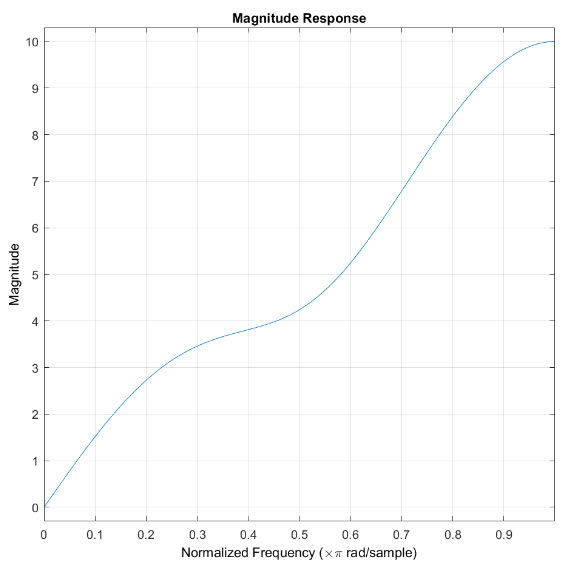
\includegraphics[width=0.8\textwidth]{images/20220217_12.png}
        \end{center}
    }

    \subsubsection{Define minimum phase filter with fixed amplitude}
    [2 pts] In case of it is a maximum phase filter provide its minimum phase version with the same magnitude response otherwise, if it is a "minimum phase filter" provide its maximum phase version.

    \mybox{
        The filter is maximum phase, the two zeros are outside the circle
        $$
        H(z)=1-z^{-1}+4z^{-2}-4z^{-3}=(z^{-1}-1)(-4z^{-2}-1)=(1-z^{-1})(1+4z^{-2})
        $$
        $$
        \begin{cases}
            \rho^2=4\\
            2\rho\cos\theta=0
        \end{cases}
        \Rightarrow
        \begin{cases}
            \rho=2\\
            \theta=\pm\frac{\pi}{2}
        \end{cases}
        $$
        Write the $G$ version of those that introduce maximum phase:
        $$
        H_m(z)=(1-z^{-1})(4+z^{-2})=4-4z^{-1}+z^{-2}-z^{-3}
        $$
    }

    \subsubsection{Output samples: convolution}
    [3 pts] Working in the time domain evaluate the output $y[n]$ of the signals
    $x_a[n]=\Brackets{1,-1,1,-1}$ and $x_b[n]=\Brackets{1,1,1,1}$ with filter $h[n]$.

    \mybox{
        $$h[n]=\delta(n)-\delta(n-1)+4\delta(n-2)-4\delta(n-3)$$
        \begin{center}
            \begin{tabular}{c|c c c c c c c}
                $n=$        & 0 & 1 &  2 &  3 & 4 & 5 & 6\\ \hline \hline
                $x_a[n]$    & 1 & -1 & 1 & -1\\
                $-x_a[n-1]$ &  0 & -1 & 1 & -1 & 1\\
                $4x_a[n-2]$ &  0 &  0 & 4 & -4 & 4 & -4\\
                $-4x_a[n-3]$&  0 &  0 & 0 &-4 &  4 &-4 & 4\\ \hline
                $y_a[n]$    &  1 & -2 & 6 &-10& 9 & -8 & 4
            \end{tabular}        
        \end{center}
        \vspace{1em}
        \begin{center}
            \begin{tabular}{c|c c c c c c c}
                $n=$        & 0 & 1 &  2 &  3 & 4 & 5 & 6\\ \hline \hline
                $x_b[n]$    & 1 &  1 & 1 &  1\\
                $-x_b[n-1]$ & 0 & -1 &-1 & -1 &-1\\
                $4x_b[n-2]$ & 0 &  0 & 4 &  4 & 4 & 4\\
                $-4x_b[n-3]$& 0 &  0 & 0 & -4 &-4 &-4 &-4\\ \hline
                $y_b[n]$    & 1 &  0 & 4 &  0 &-1 & 0 &-4
            \end{tabular}        
        \end{center}
    }

\pagebreak\subsection{20220217-2*}
    A signal $x(t)=\sin(2\pi 100t)+2\cos(2\pi 50t)$ is sampled at $400Hz$ and then downsampled by an order of $M=3$

    \subsubsection{Downsampling without LPF}
    [5pts] What is the output in case of no low pass (antialiasing) filter is adopted? Depict the magnitude of the output in the range $0-\pi$ (normalized frequencies).

    \mybox{
        $$
        F_s=400
        $$
        The sampled signal is
        $$
        x[n]=\sin(\frac{\pi}{2}n)+2\cos(\frac{\pi}{4}n)
        $$
        So after downsampling:
        $$
        x_d[n]=x[nM]=\sin(\frac{3\pi}{2}n)+2\cos(\frac{3\pi}{4}n)
        $$

    }

\pagebreak\subsection{20220126-1}
    We need to apply the first derivative ($h[n]=\Brackets{1,-1}$) in real-time to a digital signal $x[n]=\Brackets{1,2,0,1,0,1,\cdots}$ working in the frequency domain on blocks of 4 samples.

    \subsubsection{DFT}
    [4pts] Describe how to get the DFT for each block of the signal and for the filter according to the requested task.

    \mybox{
        Just use the $W$ matrix of dimension 4:
        $$
        W=
        \begin{bmatrix}
            1 & 1 & 1 & 1\\
            1 & -j & -1 & j\\
            1 & -1 & 1 & -1\\
            1 & j & -1 & -j
        \end{bmatrix}
        $$
        So the DFT of the filter will be:
        $$
        H[k]=
        \begin{bmatrix}
            1 & 1 & 1 & 1\\
            1 & -j & -1 & j\\
            1 & -1 & 1 & -1\\
            1 & j & -1 & -j
        \end{bmatrix}
        \begin{bmatrix}
            1\\
            -1\\
            0\\
            0
        \end{bmatrix}=
        \begin{bmatrix}
            0\\
            1+j\\
            2\\
            1-j
        \end{bmatrix}
        $$
    }

    \subsubsection{Overlap and save}
    [7pts] Using the overlap and save algorithm, describe how to find the output for the given signal, provide all the intermediate numerical results and the steps to obtain the final result.

    \mybox{
        Blocks of 4 samples, for overlap and save fot the first block we add $\underlabel{P}{len(h)}-1=1$ leading zeros:
        \vspace{1em}

        $
        x_1[n]=\Brackets{0,1,2,0}\\
        \\
        x_2[n]=\Brackets{0,-1,0,1}\\
        $

        \vspace{1em}
        At this point we could circular convolve with the filter then DFT, or we first DFT the blocks then circular convolve. We decide the first approach and we will get (as $h[n]=\delta[n]-\delta[n-1]$)

        $
        y_1[n]=\Brackets{0,1,1,-2,0}
        $
    }

\pagebreak\subsection{20211108-1}

    \subsubsection{Zero-pole to equation in z}

    \mybox{
        $$
        H_m(z)=1+0.49z^{-2}
        $$
    }

\pagebreak\subsection{20190910-2}
    A signal $x[n]=\Brackets{-1,-1,2,0,0,1,-2,1,0,1,1,-1}$ shall be filtered with this FIR fitler: $h[n]=\Brackets{1,-1,2}$.\\
    We need to process blocks of 4 samples of the original signal for real time processing and we want to get the result depicting all intermediate steps with these methods:

    \subsubsection{Overlap and Add}
    [4pt] Overlap and Add

    \mybox{
        Subdividing the signal in blocks of $L$ elements, in this case $L=N=4$ so we get 3 blocks:
        \vspace{1em}

        $
        x_1[n]=\Brackets{-1,-1,2,0}\\
        x_2[n]=\Brackets{0,1,-2,1}\\
        x_3[n]=\Brackets{0,1,1,-1}
        $

        \vspace{1em}
        Now we filter using convolution with $h[n]=\Brackets{1,-1,2}$
        \vspace{1em}

        $
        x[n]*h[n]=x[n]*\delta[n]+x[n]*-\delta[n-1]+x[n]*2\delta[n-2]=\\
        =\cdots x[n]-x[n-1]+2x[n-2]=\\
        $

        \begin{center}
            \begin{tabular}{c|c c c c c c}
                $n=$        & 0 & 1 &  2 &  3 & 4 & 5\\ \hline \hline
                $x_1[n]$    & -1 & -1 & 2 & 0\\
                $-x_1[n-1]$ &  0 &  1 & 1 & -2 & 0\\
                $2x_1[n-2]$ &  0 &  0 &-2 & -2 & 4 & 0\\ \hline

                $x_2[n]$    & 0 & 1  & -2 & 1\\
                $-x_2[n-1]$ & 0 &  0 & -1 & 2 &-1\\
                $2x_2[n-2]$ & 0 &  0 & 0  & 2 &-4 & 2\\ \hline

                $x_3[n]$    & 0 &  1 & 1 & -1\\
                $-x_3[n-1]$ & 0 &  0 &-1 & -1 & 1\\
                $2x_3[n-2]$ & 0 &  0 & 0 & 2  & 2 & -2

            \end{tabular}        
        \end{center}
        \vspace{1em}

        $
        \Rightarrow y_1[n]=\begin{Bmatrix}
            -1 & 0 & 1 & -4 & 4 & 0
        \end{Bmatrix}\\
        \Rightarrow y_2[n]=\begin{Bmatrix}
            0 & 1 & -3 & 5 & -5 & 2
        \end{Bmatrix}\\
        \Rightarrow y_3[n]=\begin{Bmatrix}
            0 & 1 & 0 & 0 & 3 & -2
        \end{Bmatrix}
        $

        \vspace{1em}
        Considering the overlapping tails, as:
        $$
        y[n]=x[n]*h[n]=\sum_{r=0}^\infty y_r[n-r\underlabel{L}{4}]
        $$
        $$
        \begin{bmatrix}
            -1 & 0 & 1 &-4 & 4 & 0\\
            &   &   &   & 0 & 1 &-3 & 5 &-5 & 2\\    
            &   &   &   &   &   &   &   & 0 & 1 & 0 & 0 & 3 & -2\\    
        \end{bmatrix}
        $$
        And the final result is
        $$
        y[n]=\begin{Bmatrix}
            -1 & 0 & 1 & -4 & 4 & 1 & -3 & 5 & -5 & 3 & 0 & 0 & 3 & -2
        \end{Bmatrix}
        $$
    }
    \subsubsection{Overlap and Save}
    [4pt] Overlap and Save

    \mybox{
        Subdividing the signal in blocks of $L$ elements, in this case $L=N=4$ so we get 3 blocks:
        \vspace{1em}

        $
        x_1[n]=\Brackets{-1,-1,2,0}\\
        x_2[n]=\Brackets{0,1,-2,1}\\
        x_3[n]=\Brackets{0,1,1,-1}
        $

        \vspace{1em}
        As the filter $h[n]$ has length $P=3$, we need to add $P-1=2$ "0"s at the beginning to account for the circular convolution effect, and for each $x_{i>1}$ we add the 2 samples before, hence in overlap and save
        $$L=N+P-1=4+2=6$$

        $
        x_1[n]=\Brackets{\mathbf{0,0,}-1,-1,2,0}\\
        x_2[n]=\Brackets{\mathbf{2,0,}0,1,-2,1}\\
        x_3[n]=\Brackets{\mathbf{-2,1,}0,1,1,-1}
        $

        \vspace{1em}
        Now we filter using circular convolution with $h[n]=\Brackets{1,-1,2}$. But we don't compute the circular convolution traditionally, we use this strategy:
        $$x_L\circledast h_L=\left[\underlabel{\cdots\cdots}{$P-1$ to discard}\cdots\cdots\underlabel{\cdots}{$L-1$}\right]$$
        a circular convolution of block $L$ will discard the first $P-1$ samples, then the rest till $L-1$ will be the same obtained from a normal convolution
        $$
        x[n]*h[n]=x[n]*\delta[n]+x[n]*-\delta[n-1]+x[n]*2\delta[n-2]=x[n]-x[n-1]+2x[n-2]
        $$

        \begin{center}
            \begin{tabular}{c|c c c c c c}
                $n=$        & 0 & 1 &  2 &  3 & 4 & 5\\ \hline \hline
                $x_1[n]$    & 0 & 0 & -1 & -1 & 2 & 0\\
                $-x_1[n-1]$ & 0 & 0 &  0 &  1 & 1 & -2\\
                $2x_1[n-2]$ & 4 & 0 &  0 &  0 &-2 & -2\\ \hline

                $x_2[n]$    & 2 & 0  & 0 & 1  & -2 & 1\\
                $-x_2[n-1]$ &-1 & -2 & 0 &  0 & -1 & 2\\
                $2x_2[n-2]$ &-4 & 2  & 4 &  0 & 0  & 2\\ \hline

                $x_3[n]$    & -2 & 1 & 0 &  1 & 1 & -1\\
                $-x_3[n-1]$ & 1  & 2 &-1 &  0 &-1 & -1\\
                $2x_3[n-2]$ & 2  &-2 &-4 &  2 & 0 & 2

            \end{tabular}        
        \end{center}
        \vspace{1em}
        We throw the first two as $P-1=2$, so:
        \vspace{1em}

        $
        \Rightarrow y_1[n]=\begin{Bmatrix}
            \cdot & \cdot & -1 & 0 & 1 & 4
        \end{Bmatrix}\\
        \Rightarrow y_2[n]=\begin{Bmatrix}
            \cdot & \cdot & 4 & 1 & -3 & 5
        \end{Bmatrix}\\
        \Rightarrow y_3[n]=\begin{Bmatrix}
            \cdot & \cdot & -5 & 3 & 0 & 0
        \end{Bmatrix}
        $

        \vspace{1em}
        And the final result is
        $$
        y[n]=\Brackets{y_1\,\,y_2\,\,y_3}=\begin{Bmatrix}
            -1 & 0 & 1 & 4 & 4 & 1 & -3 & 5 & -5 & 3 & 0 & 0
        \end{Bmatrix}
        $$
    }




% \begin{center}
%     \begin{tabular}{X|c c c c c c}
%         $n=1$       & 0 & 1 &  2 &  3 & 4 & 5\\ \hline
%         $x_1[n]$    & 0 & 0 & -1 & -1 & 2 & 0\\
%         $-x_1[n-1]$ & 0 & 0 &  0 &  1 & 1 & -2\\
%         $2x_1[n-2]$ & 0 & 0 &  0 &  0 &-2 & -2
%     \end{tabular}        
% \end{center}

\pagebreak\subsection{20190722-1}
    A signal $x(t)$ is sampled at $10kHz$, and we want to find the relative magnitude of its components at $1kHz$ w.r.t. the components at $4kHz$ but we \underline{cannot} use the FFT.

    Therefore we decide to filter the signal at $1kHz$ and $4kHz$ multiplying it with a real sinusoid at $1kHz$ and at $4kHz$ respectively.

    \subsubsection{Not using FFT/DFT, use a cosine and pole-zero plot}
    [3 pts] Depict the pole zero plots for the two sinusoids.

    \mybox{
        The signal is sampled at $10kHz$ so
        $$F_s=10kHz$$
        If we could use th DFT or FFT, we could just use
        $$
        X(k)=\sum_{n=0}^{N-1} x(n)e^{-j2\pi \frac{k}{N}n}\big|_{f=1kHz}
        $$
        Instead we exploit a real sinusoid in the time domain:
        $$
        s(n)=\cos(2\pi \overline{f}n)
        $$
        Whose Fourier transform will result in two pulses (two $\delta$'s) in the frequency domain as it is a cosine: in $\overline{f}$ and in $-\overline{f}$. If we compute
        $$
        X(f)\cdot DTFT(\cos(2\pi fn))\big|_{f=1kHz}=X(f=1kHz)\delta(f-1kHz)+X(f=1kHz)\delta(f+1kHz)
        $$
        As we consider normalized frequencies and compute the z-transform:
        $$f_1=1kHz\rightarrow \tilde{f}_1=\frac{f_1}{Fs}$$
        $$
        \cos\left(2\pi\frac{1kHz}{10kHz}n\right)\cdot\underlabel{u(n)}{Discrete unitary step, the signal is defined only in the positive values}
        $$
        Using
        $$
        Z\brackets{r^n\cos(\omega_0n)u(n)}=\frac{1-r\cos(\omega_0)z^{-1}}{1-2r\cos(\omega_0)z^-1+r^2z^{-2}}
        $$
        $$
        Z-TX=\frac{1-\cos(\bigslant{\pi}{5})z^{-1}}{
            1-2\cos(\bigslant{\pi}{5})z^{-1}+z^{-2}}
        $$
    }

    \mybox{
        Alternatively we convert it to the exponential form and solve the z-transform explicitely
        $$
        \begin{cases}
            \frac{e^{j\frac{\pi}{5}n}+e^{-j\frac{\pi}{5}n}}{2}\cdot u(n)\\
            X(z)=\sum_{n=-\infty}^{+\infty}x(n)\cdot z^{-n}
        \end{cases}
        $$
        So due to geometric sum:
        $$
        Z-TX(e^{j\frac{\pi}{5}n}\cdot u(n))=\sum_{n=0}^\infty e^{j\frac{\pi}{5}n}z^{-n}=\sum_{n=0}^\infty\left(e^{j\frac{\pi}{5}}z^{-1}\right)^n=\frac{1}{1-e^{j\frac{\pi}{5}z^{-1}}}
        $$
        $$
        Z-TX=\frac{1}{2}\left(\frac{1}{1-e^{j\frac{\pi}{5}z^{-1}}}+\frac{1}{1-e^{-j\frac{\pi}{5}z^{-1}}}\right)=\cdots
        $$
        From
        $$
        H_1(z)=\frac{1-\cos(\bigslant{\pi}{5})z^{-1}}{1-2\cos(\bigslant{\pi}{5})z^{-1}+z^{-2}}
        $$
        We can find the zeros and the poles
        \begin{itemize}
            \item For the denominator we exploit:
            $$
            1-2\rho\cos(\theta)z^{-1}+\rho^2z^{-2}\leftrightarrow \rho(\cos(\theta)\pm j\sin(\theta))
            $$
            Poles in $e^{\pm j\frac{\pi}{5}}$ \textbf{plus double zero in the origin}
            \item For the numerator the zeros are just the coefficients of $z^{-k}$, so we have a zero in $\cos(\frac{\pi}{5})$ \textbf{plus a pole in the origin which will cancel out with the double zero in the origin leaving a single zero}
        \end{itemize}
        \begin{center}
            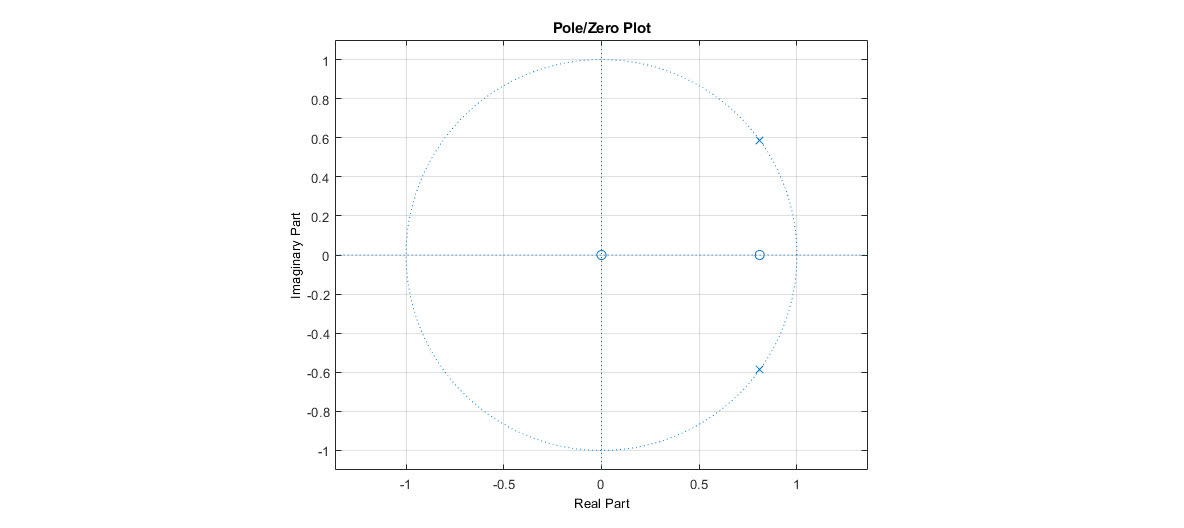
\includegraphics[width=1\textwidth]{images/20190722_01.png}
        \end{center}
        Same reasoning for $4Hz$, we will get
        $$
        H_2(z)=\frac{1-\cos(\bigslant{4\pi}{5})z^{-1}}{1-2\cos(\bigslant{4\pi}{5})z^{-1}+z^{-2}}
        $$
    }

    \subsubsection{Difference equations (anti z-transform)}
    [6 pts] Define the difference equations both for the first and the second sinusoid.

    \mybox{
        Everything at numerator will be $x$'s on the right, everything at the denominator will be $y$'s on the left:
        \vspace{1em}

        $
        H_1(z)=\frac{1-\cos(\bigslant{\pi}{5})z^{-1}}{1-2\cos(\bigslant{\pi}{5})z^{-1}+z^{-2}}\\
        \\
        y_1(n)-2\cos(\bigslant{\pi}{5})y(n-1)+y(n-2)=
        1-\cos(\bigslant{\pi}{5})x(n-1)\\
        \\
        H_2(z)=\frac{1-\cos(\bigslant{4\pi}{5})z^{-1}}{1-2\cos(\bigslant{4\pi}{5})z^{-1}+z^{-2}}\\
        \\
        y_2(n)-2\cos(\bigslant{4\pi}{5})y(n-1)+y(n-2)=
        1-\cos(\bigslant{4\pi}{5})x(n-1)\\
        $
    }

    \subsubsection{How to apply the filters}
    [3 pts] Describe how we shall apply the previously defined filters in order to measure the relative intensity of the input signal at 1kHz with respect to 4kHz.

    \mybox{
        In order to apply the filters we have to take a portion of the input signal and process it with the two filters (the difference equations above).
        
        To avoid polarizations in the measure we should take a set of samples multiple of the wavelengths (in term of samples) of both the sinusoids. 
        
        The ratio of the two magnitudes of the outputs will give the result.
    }

    \subsubsection{Cosine method weakness w.r.t. Fourier Transform}
    [1 pts] What is a weakness of the proposed system with respect to the Fourier Transform?

    \mybox{
        The weakness with respect to the Fourier Transform is related to the fact that we are not using the phase as in the Discrete Fourier Transform, so, signal components with the same amplitude and frequency but different phases will give different results.

        By multiplying our signal with a signal in the Fourier domain, it means that we are convolving the signal with a cosine:
        $$
        y(n)=\sum_mx(n-m)\cos(2\pi\underlabel{\tilde{f}}{1kHz}n)
        $$
        While the DFT:
        $$
        X(k)=\sum_{n=0}^{N-1} x(n)e^{-j2\pi \frac{k}{N}n}\big|_{f=1kHz}=
        \sum_{n=0}^{N-1} x(n)\left(\cos(2\pi fn)-j\sin(2\pi fn)\right)\big|_{f=1kHz}
        $$
        So we are not considering a sin component.
    }

\pagebreak\subsection{20190212-2}
    A signal is sampled at $10kHz$ filling all the available band. We need to upsample it to $15kHz$.

    \subsubsection{Upsample by noninteger pipeline}
    [3pts] Provide the full pipeline to properly upsample the signal minimizing the presence of artifacts or aliasing and detailing the parameters of every bock

    \mybox{
        As we upsample to a noninteger, we can:
        $$10\rightarrow 30\rightarrow 15$$
        So we first upsample by $L=3$ and then downsample by $M=2$, which means we introduce a LPF of $\Omega_c=\min\left(\frac{\pi}{3},\frac{\pi}{2}\right)=\frac{\pi}{3}$ (in other words a filter with that cutoff $H(z)\big|_{\omega_c=\frac{\pi}{3},f_c=\frac{1}{6}}$)
        \begin{center}
            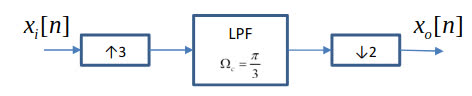
\includegraphics[width=0.8\textwidth]{images/20190212_21.png}
        \end{center}
    }

    \subsubsection{Cutoff DFT}
    [7pts] Assuming that we are working on blocks of 8 samples and we are filtering the signal in frequency domain, describe a possible implementation of the previous system working in the frequency domain (using the DFT).

    \mybox{
        8 samples, so $N=8$, after upsample we will have $8\cdot 3=24$ samples. If we have to implement that filter with that frequency and 24 samples, so
        $$
        f=\left[
            0,\frac{1}{24},\frac{2}{24},\cdots,\frac{23}{24}
        \right]
        $$
        24 samples that represent normalized frequencies, a cutoff of $f_c=\frac{1}{6}$ means that we keep the pulses till $f_c$ and introduce at the end 3 pulses (symmetry)
        \begin{center}
            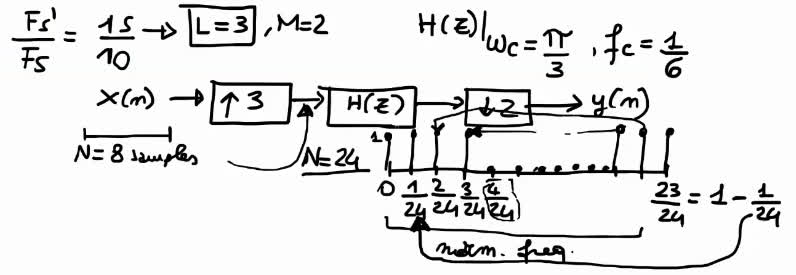
\includegraphics[width=1\textwidth]{images/20190212_22.png}
        \end{center}
    }

\pagebreak\subsection{20190116-2}
    A maximum phase filter has the following transfer function:
    $$
    H_M(z)=\frac{
        \left(
            1-2\sqrt{2}z^{-1}+4z^{-2}
        \right)
        \left(
            1+2\sqrt{2}z^{-1}+4z^{-2}
        \right)
    }{4+z^{-2}}
    $$

    \subsubsection{Zero-pole plot}
    [2 Pts.] Provide its zeros-poles plot

    \mybox{
        Poles:
        $$z^{-2}=-4\rightarrow \pm\frac{i}{2}$$
        Zeros, make sure the $\Delta<0$, otherwise we cannot use the formula for complex conjugates. In this case the condition holds, so
        $$
        1-2\rho\cos\theta z^{-1}+\rho^2 z^{-2}
        \Rightarrow
        \begin{cases}
            2\sqrt{2}=2\rho\cos\theta\\
            4=\rho^2
        \end{cases}\Rightarrow
        \begin{cases}
            \rho=2\\
            \theta=\pm\frac{\pi}{4}
        \end{cases}
        $$
        $$
        1-2\rho\cos\theta z^{-1}+\rho^2 z^{-2}
        \Rightarrow
        \begin{cases}
            -2\sqrt{2}=2\rho\cos\theta\\
            4=\rho^2
        \end{cases}\Rightarrow
        \begin{cases}
            \rho=2\\
            \theta=\pm\frac{3}{4}\pi
        \end{cases}
        $$
        We also introduced in the origin 2 zeros and 4 poles, so we will have 2 poles:
        \begin{center}
            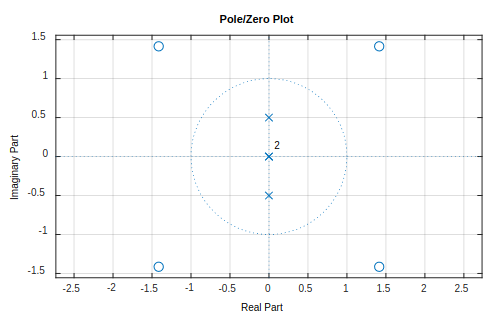
\includegraphics[width=0.7\textwidth]{images/20190116_21.png}
        \end{center}
    }

    \subsubsection{Define minimum phase filter with fixed amplitude/magnitude}
    [4 Pts.] Provide its minimum phase version, $H_m(z)$, with exactly the same magnitude response.

    \mybox{
        As $\rho=2$, now $\rho=\frac{1}{2}$:
        $$
        H_m(z)=A\frac{
            \left(
                1-\frac{\sqrt{2}}{2}z^{-1}+\frac{1}{4}z^{-2}
            \right)
            \left(
                1+\frac{\sqrt{2}}{2}z^{-1}+\frac{1}{4}z^{-2}
            \right)
        }{4+z^{-2}}
        $$
    }

    \mybox{
        Then we find $A$ by imposing:
        $$H_M(z=0)=H_m(z=0)\Rightarrow \frac{1}{4}=A\frac{1}{4}\Rightarrow A=16$$
        Alternatively write the $G$ version of those that introduce maximum phase
        $$
        H_m(z)=\frac{
            \left(
                4-2\sqrt{2}z^{-1}+z^{-2}
            \right)
            \left(
                4+2\sqrt{2}z^{-1}+z^{-2}
            \right)
        }{4+z^{-2}}
        $$
    }

    \subsubsection{Cosine signal and generic filter}
    [5 Pts.] A signal $x(t)=\cos(2\pi 1000t)$ is sampled at $4kHz$. Define the outputs $y_M[n]$ and $y_m[n]$ with the proper amplitude and phase from the two filters $H_M(z)$ and $H_m(z)$.

    \mybox{
        A cosine by a generic filter $H$ will give another cosine with different amplitude and phase.

        $f_0=1000=1kHz$, $F_s=4kHz$, so the normalized frequency $\tilde{f}_0=\frac{f_0}{F_s}=\frac{1}{4}$ and $\tilde{\omega}_0=\frac{\pi}{2}$

        In the z-transform we will have (we always consider the normalized!):
        $$
        z_0=1*e^{j\omega}=e^{j2\pi f}=e^{j\pi/2}=j
        $$
        \begin{itemize}
            \item Maximum phase
            $$
            H_M(z)\rightarrow\begin{cases}
                \left|H_M(z=j)\right|=\cdots=\frac{17}{3}\\
                \angle H_M(z=j)=\angle
                H_M(z)=\frac{
                    \left(
                        1-2\sqrt{2}j^{-1}-4
                    \right)
                    \left(
                        1+2\sqrt{2}j^{-1}-4
                    \right)
                }{4-1}
            \end{cases}
            $$
            The phase:
            $$
            \angle
                H_M(z)=\frac{
                    \left(
                        2\sqrt{2}j-3
                    \right)
                    \left(
                        -2\sqrt{2}j-3
                    \right)
                }{3}
                =
                \angle(-3+2\sqrt{2}j)+\angle(-3-2\sqrt{2}j)+\angle(3)
            $$
            The phase of a real number is zero in the complex plane, while the phase of the first term will be in the third quadrant and the phase of the second term will be the first mirrored, so summing them together will get $\angle H_M(j)=2\pi$
            $$y_M(n)=A\cdot\cos(\tilde{\omega}_0n+\phi)=\frac{17}{3}\cos(\frac{\pi}{2}n+2\pi)$$
            \item Minimum phase, as we \textbf{imposed that the magnitude is the same}
            $$
            H_m(z)\rightarrow\begin{cases}
                \left|H_m(z=j)\right|=\left|H_M(z=j)\right|=\frac{17}{3}\\
                \angle H_M(z=j)=\angle
                \frac{
                    \left(
                        3+2\sqrt{2}j
                    \right)
                    \left(
                        3-2\sqrt{2}j
                    \right)
                }{3}
                =
                0
            \end{cases}
            $$
            The phase is 0 as the phase of the first is in the first quadrant $\angle H_m(j)=0$
            $$y_m(n)=A\cdot\cos(\tilde{\omega}_0n+\phi)=\frac{17}{3}\cos(\frac{\pi}{2}n+0)$$
        \end{itemize}
    }

\pagebreak\subsection{20181107-1}
    An analog signal $x(t)=2\cos(2\pi 20t)+3\sin(2\pi 60t)+4\cos(2\pi 80t)$ is sampled at 160 samples/s and filtered with an IIR filter with the following finite differences equation:
    $$
    y[n]=x[n]+\sqrt{2}x[n-1]+x[n-2]-0.9\sqrt{2}[n-1]-0.81y[n-2]
    $$

    \subsubsection{Z-transform and pole-zero plot}
    [2pts] Provide the z-transform of the filter.

    [3pts] Provide the zeros-poles plot of the filter.

    \mybox{
        $$F_s=160$$
        So the sampled signal is
        $$
        x(t)=2\sin(\frac{\pi}{4} n)+3\cos(\frac{3\pi}{4}n)+4\sin(\pi n)
        $$
        $$
        H(z)=\frac{
            1+\sqrt{2}z^{-1}+z^{-2}
        }{
            1+0.9\sqrt{2}z^{-1}+0.81z^{-2}
        }
        $$
        \begin{itemize}
            \item Numerator:
            $$
            \begin{cases}
                \rho^2=1\\
                2\rho\cos\theta=-\sqrt{2}
            \end{cases}
            \Rightarrow
            \begin{cases}
                \rho=1\\
                \theta=\pm\frac{3\pi}{4}
            \end{cases}
            $$
            Two zeros in $e^{\pm j\frac{3\pi}{4}}$, two poles in 0
            \item Denominator:
            $$
            \begin{cases}
                \rho^2=0.81\\
                2\rho\cos\theta=-0.9\sqrt{2}
            \end{cases}
            \Rightarrow
            \begin{cases}
                \rho=0.9\\
                \theta=\pm\frac{3\pi}{4}
            \end{cases}
            $$
            Two poles in $0.9e^{\pm j\frac{3\pi}{4}}$, two zeros in 0
        \end{itemize}
        So no zeros or poles at the origin, system stable as all poles and zero in the circle:
        \begin{center}
            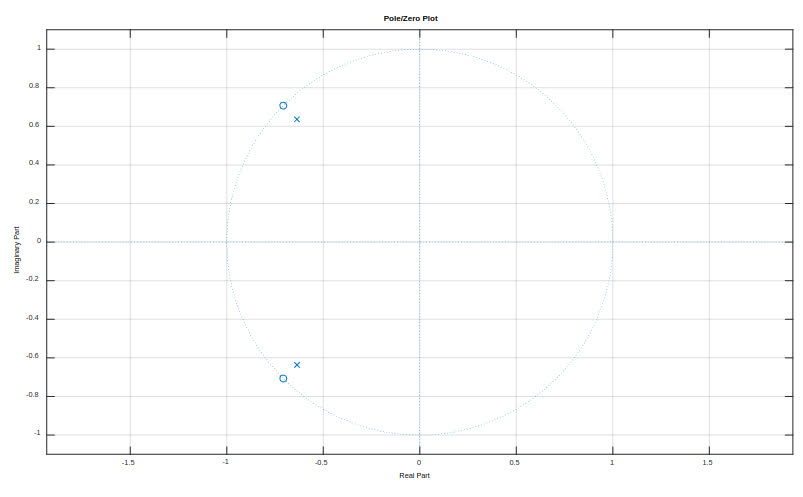
\includegraphics[width=0.9\textwidth]{images/20181107_11.png}
        \end{center}
    }

    \subsubsection{Magnitude and phase plot by hand}
    [3pts] Represent an approximate behavior of the magnitude and phase in the range $(0\,\,-\pi)$.

    \mybox{
        $$
        H(z)=\frac{
            1+\sqrt{2}z^{-1}+z^{-2}
        }{
            1+0.9\sqrt{2}z^{-1}+0.81z^{-2}
        }
        $$
        The range is normalized in $(0\,\,1)$. We start from the magnitude, we compute some notable points:
        \begin{itemize}
            \item $|H(z=1,\omega=0)|=\frac{2+\sqrt{2}}{1.81+0.9\sqrt{2}}\sim 1.1075$
            \item $|H(z=j,\omega=\pi/2)|=\left|\frac{-\sqrt{2}j}{0.19-0.9\sqrt{2}j}\right|=\frac{\sqrt{2}}{\sqrt{0.19^2+0.81*2}}\sim 1.0989$
            \item $|H(z=e^{-j\frac{3\pi}{4}},\omega=3\pi/4)|=0$, as in that angle we meet the zero so we are multiplying by 0
            \item $|H(z=-1,\omega=\pi)|=\frac{2-\sqrt{2}}{1.81-0.9\sqrt{2}}\sim 1.0904$
        \end{itemize}
        \begin{center}
            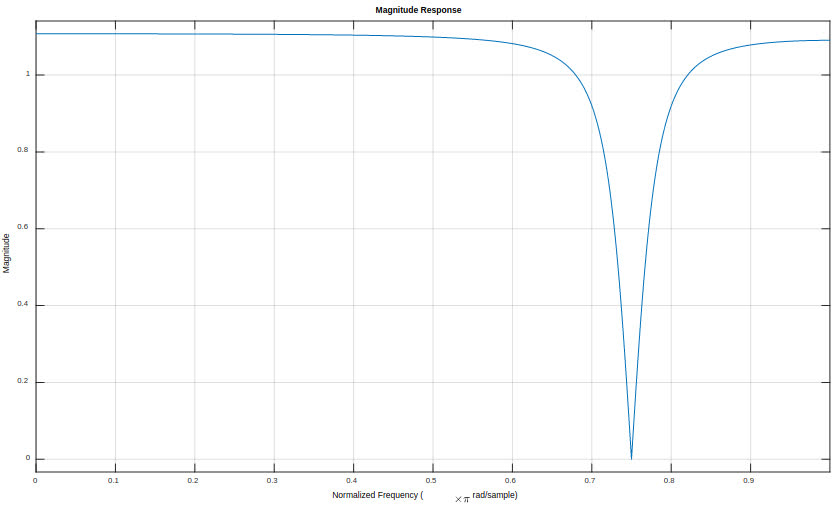
\includegraphics[width=0.8\textwidth]{images/20181107_12.png}
        \end{center}

        About the phase, we have to look at the zero plot:
        \begin{itemize}
            \item $\angle H(z=1)=0$ as we have opposite contributes for both poles and zeros
            \item $\angle H(z=e^{-j\frac{3\pi}{4}})$ we don't know the exact value, but at that pole we will have a jump of $\pi$
            \item $\angle H(z=-1)=0$ as we have opposite contributes for both poles and zeros
        \end{itemize}
        \begin{center}
            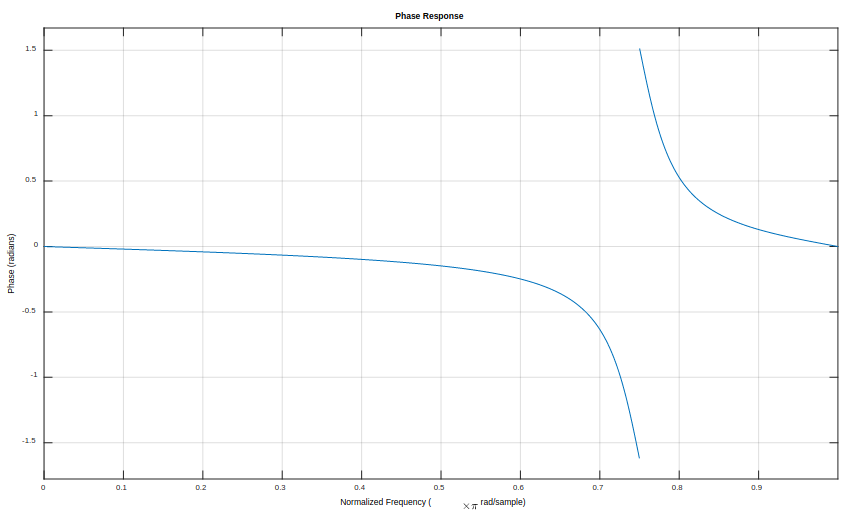
\includegraphics[width=0.8\textwidth]{images/20181107_13.png}
        \end{center}
    }

    \subsubsection{Sampled signal, cosine signal and generic filter}
    [5pts] What will be the discrete output signal when the input is the sampled version of $x(t)$

    \mybox{
        $$F_s=160$$
        The signal is
        $$
        x(t)=2\cos(2\pi 20t)+3\sin(2\pi 60t)+4\cos(2\pi 80t)
        $$
        It has three components, so:
        \begin{itemize}
            \item $\tilde{f_1}=\frac{f_1}{F_s}=\frac{20}{160}=\frac{1}{8}\rightarrow\tilde{\omega}_1=\frac{\pi}{4}\rightarrow z_1=1*e^{j\pi/4}$
            $$
            \begin{cases}
                |H(z_1)|=\cdots=1.1068\\
                \angle H(z_1)=\cdots=-0.053
            \end{cases}
            $$
            \item $\tilde{f_2}=\frac{f_2}{F_s}=\frac{60}{160}=\frac{3}{8}\rightarrow\tilde{\omega}_2=\frac{3\pi}{4}\rightarrow z_2=1*e^{j3\pi/4}$
            $$
            \begin{cases}
                |H(z_2)|=0\\
                \angle H(z_2)=\text{ does not matter, the magnitude is 0 so the term disappears}
            \end{cases}
            $$
            \item $\tilde{f_3}=\frac{f_3}{F_s}=\frac{80}{160}=\frac{1}{2}\rightarrow\tilde{\omega}_3=\pi\rightarrow z_3=1*e^{j\pi}=-1$
            $$
            \begin{cases}
                |H(z_3)|=1.0904\\
                \angle H(z_3)=0
            \end{cases}
            $$
        \end{itemize}
        The output is:
        $$
        y[n]=2\cdot 1.1065\cos\left(\frac{\pi}{4}n-0.053\right)+4\cdot 1.09\cos(\pi n)
        $$
    }

\pagebreak\subsection{20160223-1}
    A filter $H_1(z)$ presents the following zero-pole plot:
    \begin{center}
        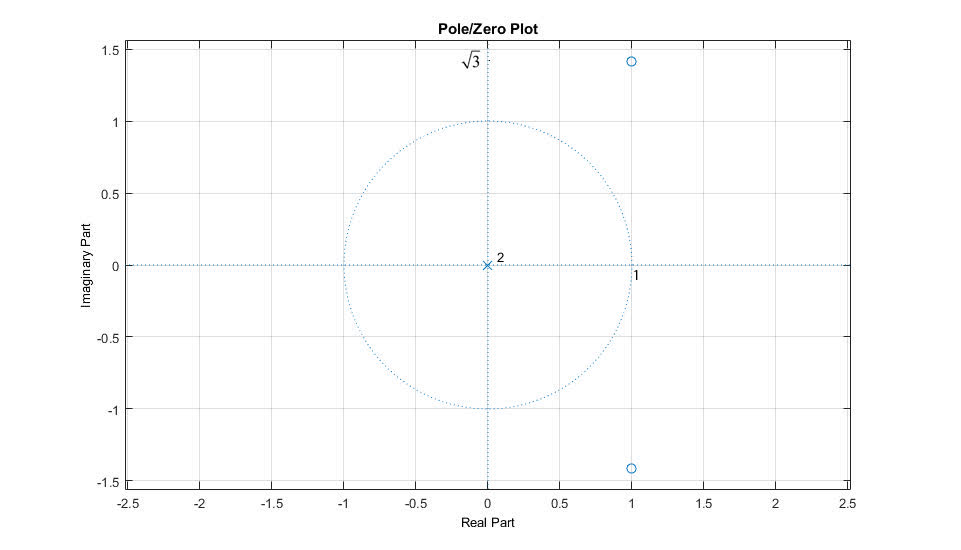
\includegraphics[width=1\textwidth]{images/20160223_01.png}
    \end{center}
    Where the two zeros are in $1\pm\sqrt{3}j$

    \subsubsection{Define minimum phase filter with fixed amplitude}
    Define a minimum phase filter $H_2(z)$ with \textbf{exactly} the same amplitude response

    \mybox{
        As two zeros are outside, we are dealing with maximum phase filter: we want to bring the zeros inside keeping the same amplitude, so we must \textbf{move zeros to their complex conjugate position, inside the circle}.\\
        For example the zero on top-right has distance $\sim 2$, we move it inside the same distance segment closer to origin till distance=$2^{-1}$, then we flip it w.r.t. x-axis.\\
        A couple of conjugate zeros with \textbf{negative $\rho$}, so we use:
        $$
        1-2\rho\cos(\theta)z^{-1}+\rho^2z^{-2}\leftrightarrow \rho(\cos(\theta)\pm j\sin(\theta))
        $$
        $$
        H_1(z)=1-2\rho\underlabel{\frac{1}{2}}{Cosine of $\theta$ for zero at $+\sqrt{3}$}z^{-1}+\rho^2z^{-2}=-2\cdot 2\frac{1}{2}z^{-1}+2^2z^{-2}
        $$
        $$
        H_1(z)=1-2z^{-1}+4z^{-2}
        $$
        Consider the conjugate (we put $\rho=2^{-1}=\frac{1}{2}$)
        $$
        H_2(z)=A\left(1-\frac{1}{2}z^{-1}+\frac{1}{4}z^{-4}\right)
        $$
    }

    \mybox{
        This is the minimum phase filter. Imposing:
        $$
        H_1(z=1,\omega=0)=H_2(z=1)\Rightarrow 3=A\cdot\frac{3}{4}\Rightarrow A=4
        $$
        \begin{center}
            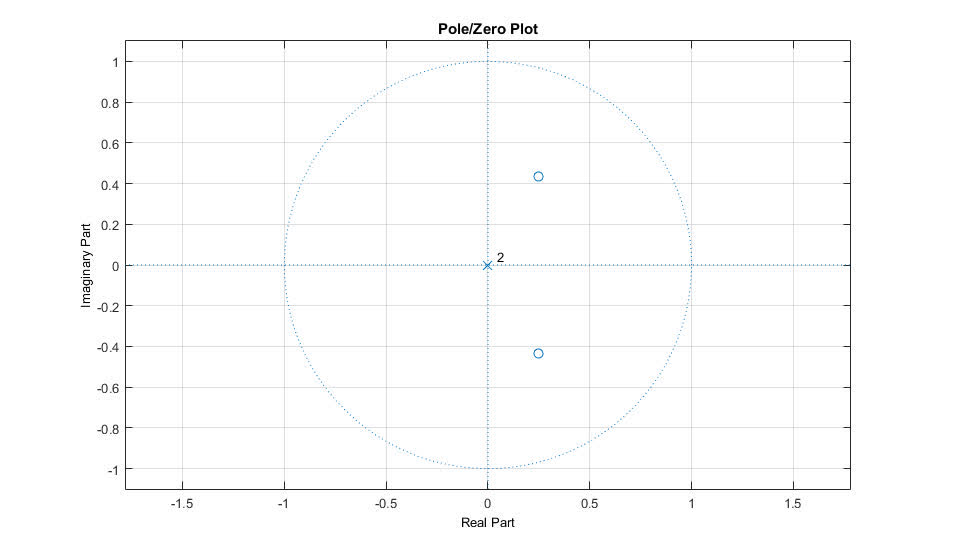
\includegraphics[width=1\textwidth]{images/20160223_02.png}
        \end{center}

        Magnitude is the same but with a different gain
        \begin{center}
            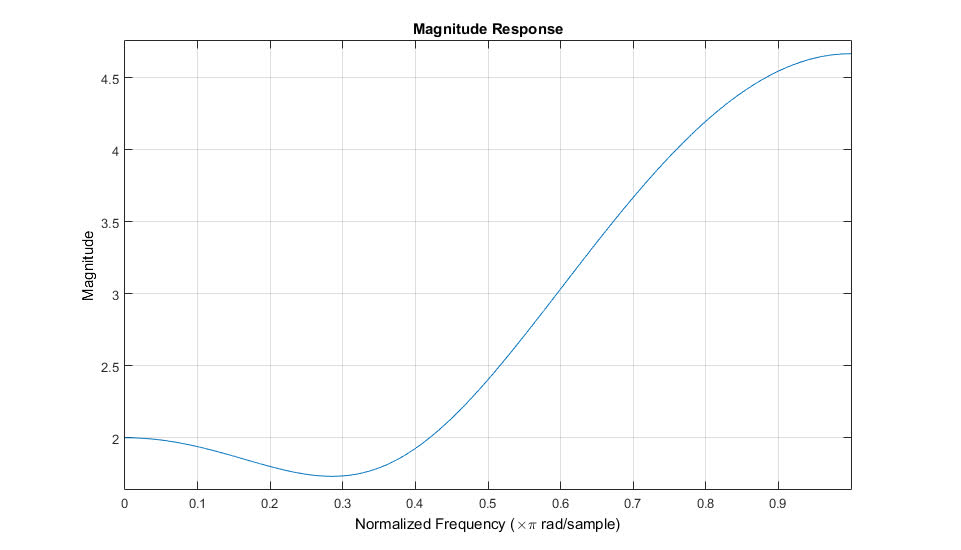
\includegraphics[width=1\textwidth]{images/20160223_03.png}
        \end{center}
    }

    \subsubsection{IIR filter to remove effect}
    Define a pure IIR filter $H_3(z)$ that, placed after the filter $H_2(z)$ is able to completely remove its effect

    \mybox{
        Remove the zeros
        $$
        H_3(z)=4\frac{1}{
            1-\frac{1}{2}z^{-1}+\frac{1}{4}z^{-2}
        }=4H_2(z)^{-1}
        $$
    }

    \subsubsection{Output samples}
    Find the first five output samples of the filters $H_1(z),H_2(z),H_3(z)$

    \mybox{
        $$
        x[n]=\delta[n]
        $$
        $$
        y_1[n]=x[n]-2x[n-1]+4x[n-2]
        $$
        So: \Brackets{1,-2,4}. For $y_2$ solve similarly. For $y_3$:
        $$
        y_3[n]=4\left(
            \frac{1}{2}y[n-1]-\frac{1}{4}y[n-2]
        \right)+x[n]
        $$
    }

\pagebreak\subsection{20160223-2}
    We want to remove the continuous component (zero frequency) from the periodic signal $x(n)$ represented below just working with the DFT.
    \begin{center}
        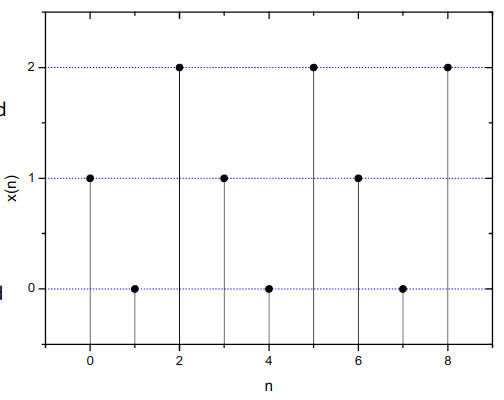
\includegraphics[width=0.7\textwidth]{images/20160223_05.png}
    \end{center}

    \subsubsection{DFT to remove continuous component}
    Propose a filter $H(k)$ in the frequency domain and apply it to the signal (provide also the $W$ matrix).

    \mybox{
        From the picture we can deduce:
        $$x(n)=\delta(n)+2\delta(n-2)$$
        With period 3. Reminder, the $W$ matrix is
        $$
        W=
        \begin{bmatrix}
            W_i^0 & W_i^0 & W_i^0 & W_i^0 & \cdots & W_i^n\\
            W_i^0 & W_i^1 & W_i^2 & W_i^3 & \cdots & W_i^{n-1}\\
            W_i^0 & W_i^2 & W_i^4 & W_i^6 & \cdots & W_i^{2(n-1)}\\
            W_i^0 & W_i^3 & W_i^6 & W_i^9 & \cdots & W_i^{3(n-1)}\\
            \vdots & \vdots & \vdots & \vdots & \ddots & \vdots\\
            W_i^0 & W_i^{n-1} & W_i^{2(n-1)} & W_i^{3(n-1)} & \cdots & W_i^{(n-1)^2}        
        \end{bmatrix}
        $$
        Where $W_i=e^{-j\frac{2\pi}{i}}$. In our case $i=3$
        $$W=
        \begin{bmatrix}
            1 & 1 & 1\\
            1 & -\frac{1}{2}-j\frac{\sqrt{3}}{2} & -\frac{1}{2}+j\frac{\sqrt{3}}{2}\\
            1 & -\frac{1}{2}+j\frac{\sqrt{3}}{2} & -\frac{1}{2}-j\frac{\sqrt{3}}{2}
        \end{bmatrix}
        $$
    }

    \mybox{
        So the DFT of x(n) will be:
        $$
        X(k)=
        \begin{bmatrix}
            1 & 1 & 1\\
            1 & -\frac{1}{2}-j\frac{\sqrt{3}}{2} & -\frac{1}{2}+j\frac{\sqrt{3}}{2}\\
            1 & -\frac{1}{2}+j\frac{\sqrt{3}}{2} & -\frac{1}{2}-j\frac{\sqrt{3}}{2}
        \end{bmatrix}
        \begin{bmatrix}
            1\\
            0\\
            2
        \end{bmatrix}=\begin{bmatrix}
            3\\
            \sqrt{3}j\\
            -\sqrt{3}j
        \end{bmatrix}
        $$
        As we want to remove the continuous component, we want to put 3 to 0 (the conjugates are 1 frequency), so we choose a
        $$H(k)=\begin{bmatrix}
            0\\
            1\\
            1
        \end{bmatrix}$$
        Applying it to the signal:
        $$Y(k)=X(k)\cdot H(k)=\begin{bmatrix}
            0\\
            \sqrt{3}j\\
            -\sqrt{3}j
        \end{bmatrix}$$
    }

    \subsubsection{DFT matrix inverse, output in time domain}
    Provide also the output in time domain $y(n)$ and a period of the filter in the time domain $h(n)$.

    \mybox{
        The inverse of $W$ is its conjugate transpose divided by $N=3$:
        $$
        W=
        \begin{bmatrix}
            1 & 1 & 1\\
            1 & -\frac{1}{2}-j\frac{\sqrt{3}}{2} & -\frac{1}{2}+j\frac{\sqrt{3}}{2}\\
            1 & -\frac{1}{2}+j\frac{\sqrt{3}}{2} & -\frac{1}{2}-j\frac{\sqrt{3}}{2}
        \end{bmatrix}
        \rightarrow
        W^{-1}=
        \frac{1}{3}
        \begin{bmatrix}
            1 & 1 & 1\\
            1 & -\frac{1}{2}+j\frac{\sqrt{3}}{2} & -\frac{1}{2}-j\frac{\sqrt{3}}{2}\\
            1 & -\frac{1}{2}-j\frac{\sqrt{3}}{2} & -\frac{1}{2}+j\frac{\sqrt{3}}{2}
        \end{bmatrix}
        $$
        $$
        y(n)=W^{-1}\cdot Y(k)=
        \frac{1}{3}
        \begin{bmatrix}
            1 & 1 & 1\\
            1 & -\frac{1}{2}+j\frac{\sqrt{3}}{2} & -\frac{1}{2}-j\frac{\sqrt{3}}{2}\\
            1 & -\frac{1}{2}-j\frac{\sqrt{3}}{2} & -\frac{1}{2}+j\frac{\sqrt{3}}{2}
        \end{bmatrix}
        \begin{bmatrix}
            0\\
            \sqrt{3}j\\
            -\sqrt{3}j
        \end{bmatrix}=
        \begin{bmatrix}
            0\\
            -1\\
            1
        \end{bmatrix}
        $$
        $$
        h(n)=W^{-1}\cdot H(k)=
        \frac{1}{3}
        \begin{bmatrix}
            1 & 1 & 1\\
            1 & -\frac{1}{2}+j\frac{\sqrt{3}}{2} & -\frac{1}{2}-j\frac{\sqrt{3}}{2}\\
            1 & -\frac{1}{2}-j\frac{\sqrt{3}}{2} & -\frac{1}{2}+j\frac{\sqrt{3}}{2}
        \end{bmatrix}
        \begin{bmatrix}
            0\\
            1\\
            1
        \end{bmatrix}=
        \begin{bmatrix}
            0\\
            -1/3\\
            -1/3
        \end{bmatrix}
        $$
    }

\pagebreak\subsection{20110202-1}
    Consider a signal made of infinite repertition of the following 4 samples: $\brackets{0;1;2;3}$

    \subsubsection{DFT}
    [4pts] Define the DFT matrix and provide the 4 Fourier coefficients for this signal

    \mybox{
        $$
        W_4=e^{-j\frac{2\pi}{4}}=e^{-j\frac{\pi}{2}}
        $$
        $$
        W=\begin{bmatrix}
            W_4^0 & W_4^0 & W_4^0 & W_4^0\\
            W_4^0 & W_4^1 & W_4^2 & W_4^3\\
            W_4^0 & W_4^2 & W_4^4 & W_4^6\\
            W_4^0 & W_4^3 & W_4^6 & W_4^9
        \end{bmatrix}=
        \begin{bmatrix}
            1 & 1 & 1 & 1\\
            1 &-j &-1 & j\\
            1 &-1 & 1 &-1\\
            1 & j &-1 &-j
        \end{bmatrix}
        $$
        $$
        X(k)=Wx=
        \begin{bmatrix}
            1 & 1 & 1 & 1\\
            1 &-j &-1 & j\\
            1 &-1 & 1 &-1\\
            1 & j &-1 &-j
        \end{bmatrix}
        \begin{bmatrix}
            0\\
            1\\
            2\\
            3
        \end{bmatrix}=
        \begin{bmatrix}
            6\\
            -2+2j\\
            -2\\
            -2-2j
        \end{bmatrix}
        $$
    }

    \subsubsection{Output samples: convolution}
    [4pts] An high pass filter, whose z-transform is $1-z^{-1}$ is applied to the signal, what will be the samples of the fitlered signal?

    \mybox{
        $$
        h[n]=\delta[n]-\delta[n-1]
        $$
        \textbf{Careful, the signal is PERIODIC, so}
        $$
        x[n-1]=\Brackets{3;0;1;2;3}
        $$
        And
        $$
        x[n]*h[n]=\Brackets{-3;1;1;1;-3}
        $$
    }

    \subsubsection{DFT}
    [4pts] What will be the DFT of the final signal?

    \mybox{
        $$
        \begin{bmatrix}
            1 & 1 & 1 & 1\\
            1 &-j &-1 & j\\
            1 &-1 & 1 &-1\\
            1 & j &-1 &-j
        \end{bmatrix}
        \begin{bmatrix}
            -3\\
            1\\
            1\\
            1
        \end{bmatrix}=
        \begin{bmatrix}
            0\\
            -4\\
            -4\\
            -4
        \end{bmatrix}
        $$
        Or compute the DFT of the filter $h$ and then multiply element-wise $y$ and $h$
    }